\documentclass{article}

\usepackage{lmodern}
\usepackage[T1]{fontenc}
\usepackage[utf8]{inputenc}

% Drafting

\usepackage[latexmk]{lwarp}

\usepackage{xcolor,soul}
\usepackage{fullpage}
\usepackage{setspace}
\usepackage{blindtext}
\doublespacing

\definecolor{mwcolor}{HTML}{8af67d}
\definecolor{vgcolor}{HTML}{c88bff} % MPL purple
\definecolor{citecolor}{HTML}{c696f0} % MPL purple


% Tools for leaving todo notes around
\usepackage[colorinlistoftodos]{todonotes}
%% \renewcommand{\todo}{}
%% \renewcommand{\hl}[1]{#1}
\newcommand{\citeme}[1]{%
  \todo[color=citecolor]{%
  \ifstrempty{#1}{[citation needed]}{[cite: #1]}%
  }%
}
\newcommand{\mw}[2]{%
  \sethlcolor{mwcolor}\hl{#2}\sethlcolor{yellow}%
  \ifstrempty{#1}{}{%
    \todo[color=mwcolor]{#1 [MW]}%
  }%                  
}
\newcommand{\vg}[2]{%
  \sethlcolor{vgcolor}\hl{#2}\sethlcolor{yellow}%
  \ifstrempty{#1}{}{%
    \todo[color=vgcolor]{#1 [VG]}%
  }%                  
}


\usepackage{graphicx}
\usepackage[version=4]{mhchem}
\usepackage{siunitx}
\usepackage[hidelinks]{hyperref}
\usepackage{glossaries}
\usepackage[xr,user]{zref} % For cross references to supplemental figures
\usepackage{textgreek}

\newcommand{\nca}[1]{\ce{Li_{#1}Ni_{0.8}Co_{0.15}Al_{0.05}O_2}}
\DeclareRobustCommand{\nmc}[2][]{%
    \ifstrempty{#1}{%
        \ce{Li_{#2}Ni_{y}Mn_{z}Co_{1-y-z}O2}}{}%
    \ifstrequal{#1}{333}{%
        \ce{Li_{#2}Ni_{1/3}Mn_{1/3}Co_{1/3}O2}}{}%
    \ifstrequal{#1}{532}{%
        \ce{Li_{#2}Ni_{0.5}Mn_{0.3}Co_{0.2}O2}}{}%
}

% Techniques
\newacronym{xrd}{PXRD}{powder X-ray diffraction}
\newacronym{uxrd}{µ-XRD}{X-ray microdiffraction}
\newacronym{txm}{TXM}{transmission X-ray microscopy}
\newacronym{xas}{XAS}{X-ray absorbance spectroscopy}
\newacronym{xanes}{XANES}{X-ray absorbance near edge spectroscopy}
\newacronym{iscat}{iSCAT}{optical interferometric scattering microscopy}

% Facilities and organizations
\newacronym{ssrl}{SSRL}{Stanford Synchrotron Radiation Lightsource}

% Chemistry
%\newacronym{ecd}{ECD}{exchange current density}
\newacronym{ecd}{$i_0$}{exchange current density}
\newacronym{od}{OD}{optical depth}
\newacronym{ocv}{OCV}{open circuit voltage}

% Particles in u-XRD mapping
\newacronym{p1}{P1}{particle 1}
\newacronym{p2}{P2}{particle 2}
\newacronym{p3}{P3}{particle 3}


\usepackage{authblk}

\title{Origin of Rapid Delithiation In Secondary Particles Of \nca{} and \nmc{} Cathodes}

\author[1,2,3]{Mark Wolfman}
\author[1]{Brian M.\ May}
\author[4]{Vishwas Goel}
\author[4]{Sicen Du}
\author[5,6]{Young-Sang Yu}
\author[7]{Nicholas V.\ Faenza}
\author[7]{Nathalie Pereira}
\author[8]{Antonin Grenier}
\author[3]{Kamila M.\ Wiaderek}
\author[3]{Ruqing Xu}
\author[9]{Jiajun Wang}
\author[8]{Karena W.\ Chapman}
\author[7]{Glenn G. Amatucci}
\author[4]{Katsuyo Thornton}
\author[1]{Jordi Cabana\thanks{Corresponding author: jcabana@uic.edu}}

\affil[1]{Department of Chemistry, University of Illinois at Chicago}
\affil[2]{Chemical Sciences and Engineering Division, Argonne National Laboratory}
\affil[3]{X-ray Science Division, Advanced Photon Source, Argonne National Laboratory}
\affil[4]{Department of Materials Science and Engineering, University of Michigan}
\affil[5]{Department of Physics, Chungbuk National University}
\affil[6]{Advanced Light Source, Lawrence Berkeley National Laboratory}
\affil[7]{Energy Storage Research Group, Department of Materials Science and Engineering, Rutgers, The State University of New Jersey}
\affil[8]{Department of Chemistry, Stony Brook University}
\affil[9]{Harbin Institute of Technology}

\date{}


\newlength{\figwidth}
\setlength{\figwidth}{3.5in}

\myexternaldocument[si:]{supplement}

\begin{document}

\maketitle

\begin{abstract}
  Most research on the electrochemical dynamics in battery materials
  has focused on the global behavior of the electrode. There has been
  debate within recent literature on the origin of an apparent
  two-phase transformation within layered cathodes for Li-ion
  batteries. The work presented here uses nano-focused X-ray probes to
  measure delithiation \textit{in operando} at the scale of secondary
  particle agglomerates in \nca{} and \nmc{} cathodes during
  charge. After an initial latent phase, individual secondary
  particles undergo rapid, stochastic, and largely uniform
  delithiation, which is in contrast with the gradual increase in
  potential measured for the whole cell. These results provide direct
  evidence that the apparent two-phase transition is emergent from
  kinetic limitations governing a population of secondary
  particles. Physics-based modeling further shows that to reproduce
  the experimental results, an
  increase in \gls{ecd} over three orders of magnitude is required during delithiation. 
  The specifics and implications of this jump
  in \gls{ecd} are crucial to understanding the charge-storage
  reaction of Li-ion battery cathodes.
\end{abstract}

\listoftodos

%%%%%%%%%%%%%%%%%%%%%%%
\section{Introduction}
%%%%%%%%%%%%%%%%%%%%%%%

% NCA/NMC material
Layered transition metal oxides represent the state-of-the-art of
cathodes materials for electrochemical energy storage. In order to
meet ever more ambitious performance targets, it will be necessary to
improve their efficiency and reliability beyond current
limitations. While layered cathodes provide high theoretical capacity,
only \SI{\approx70}{\percent} is realistically achievable, with a
steeper penalty imposed at higher rates\citeme{}. This observation
points to kinetic barriers preventing full utilization of the
cathode. Careful observation of local heterogeneity, combined with
detailed simulation of the underlying electrochemical processes, can
reveal details of the kinetic factors governing these reactions,
ultimately leading to higher performing energy storage systems. 

% TXM/XRD background

Synchrotron X-ray characterization provides several methods to
evaluate heterogeneity within secondary particles of layered cathode
materials. \Gls{uxrd} extends the structural characterization of
conventional \gls{xrd} with improved spatial resolution. Incoming
X-rays are focused to a sub-micron spot and scanned over individual
secondary particles. At each mapping position, the diffraction pattern
captured by an area detector provides details of the crystal
structure, such as the unit-cell parameters, which can then be related
to chemical states (e.g.\ extent of lithiation). A complementary
technique, \Gls{txm}, produces projection micrographs showing the
optical depth of the object with \SI{\approx30}{nm} spatial
resolution, depending on the instrument configuration. The tunable
nature of synchrotron X-ray sources allows micrographs of the same
field of view to be captured at several energies. To produce chemical
maps, images are collected at a range of energies spanning an X-ray
absorption edge, producing a separate spectrum for each pixel in the
field of view and, after data reduction, a chemical map with chemical
significance (e.g.\ metal oxidation states). For both techniques,
since the individual measurements are projections through the
specimen, the resulting maps show the average state through the
optical axis (perpendicular to the image plane).

The high transmission provided by hard X-rays is conducive to making
measurements inside an assembled cell (is-situ) and, ideally, while
the cell is actively cycling (operando). In addition to avoiding
relaxation effects, in-situ measurement allows the same object to be
measured repeatedly at different states of charge. Tracking the same
object during a (dis)charge cycle allows for a direct comparison
between different states of charge and provides a clearer picture of
how heterogeneity evolves.

%% NCA/NMC background

Ensemble \gls{xrd} has shown a mixture of phases in \nca{} electrodes
during the first charge when stored in ambient conditions, in contrast
with the solid-solution, single-phase transformation seen during
subsequent charge cycles\cite{robert2015}. A possible origin is the
presence of a lithium diffusion barrier arising from surface
\ce{Li2CO3} formation upon exposure to \ce{CO2} and \ce{H2O}. When
pristine \nca{} was protected from ambient air exposure, a
single-phase solid-solution reaction was observed during first
charge\cite{grenier2017}. This observation led to the conclusion that
the secondary particles contained an uneven coating of \ce{Li2CO3},
which must be broken electrochemically before the reaction can
proceed. The need to break this coating would produce different
timelines for reaction initiation in different particles, resulting in
a bimodal distribution of oxidation states and the appearance of
non-equilibrium heterogeneity by \gls{xrd}.

The oxidation states of individual secondary particles were measured
by operando \gls{txm} \gls{xas} and, indeed, particles were observed
to be either in a pristine or partially oxidized state with more
particles becoming oxidized at higher states of
charge\cite{nowack2016}. While \ce{Li2CO3} clearly plays a role in the
ability of lithium to penetrate into the secondary particle, it was
also demonstrated that the presence of two phases by \gls{xrd} is
suppressed by stronger compaction of the electrode during laminate
preparation\cite{bobrikov2018}. A related layered cathode material,
\nmc[333]{}, is less prone to \ce{Li2CO3} formation, even showing
lower levels of \ce{Li2CO3} after one month of air exposure than those
found in pristine \nca{}\cite{shizuka2007}. In-situ \gls{xrd} studies
of \nmc[333]{} during first charge show a largely single-phase
(solid-solution) transformation \cite{hulzen2018,ahn2017,zhou2016-2},
though some studies reveal two crystallographic phases with a small
difference in \emph{a} and \emph{c} unit-cell parameters and
coexisting over a narrow range of delithiation compared to
\nca{}\cite{yoon2006,hua2018}. The oxidation dynamics of these layered
cathode materials warrant further study to clarify the nature of the
chemical transformation, especially in view of locating the onset and
progression of heterogeneity, within and between the secondary
particles that typically compose a cathode. It is important to
elucidate how general this behavior is among the general class of
layered oxides that are leading candidates as battery materials.

This work further examined the heterogeneities present in secondary
particles of established layered cathode materials, namely \nca{},
\nmc[333]{}, and \nmc[532]{}. A combination of operando \gls{uxrd} and
\gls{txm} \gls{xas} experiments probed both the inter-particle
heterogeneity. While the cell potential and prior reports of ensemble
\gls{xas} indicated a smooth transition to higher oxidation state upon
delithiation\cite{deb2005,muto2009}, individual particles exhibited a
sharp and stochastic transition from an initial, latent state to one
containing highly oxidized \ce{Ni}. Physics-based simulations were then
conducted to determine the role of fundamental electrochemical
processes in generating this rapid delithiation behavior, which showed that this behavior due to a significant increase in the \gls{ecd} covering several orders
of magnitude during delithiation. These observations highlight the decoupling and interaction between single particle dynamics and the macroscopic response in battery electrodes even when they follow mechanisms of solid solution. The identification of \gls{ecd} as controlling parameter in these materials redirects models away from a focus on mass diffusion. 

%%%%%%%%%%%%%%%%%%%%%%%%%%%%%%%%%%%%%%%%%%%%%%%%%
\section{Operando observations of single particle dynamics}
%%%%%%%%%%%%%%%%%%%%%%%%%%%%%%%%%%%%%%%%%%%%%%%%%

%% \subsection{\Gls{uxrd} - Interparticle Dynamics}

Secondary particles of \nca{} were tracked during their
first change and discharge using operando \gls{uxrd} mapping. Dilute (\SI{20}{\percent}) \nca{} electrodes were use to isolate the response of individual particles from each other. For each
X--Y mapping position, the individual 2D diffraction signals were integrated to one-dimensional patterns. While data was collected at resolutions, ~500 nm, below the size of the particles, for the purpose of our analyses, all patterns from the same individual particle at a given time stamp during the reaction were summed (Figures \ref{fig:uxrd}a,b and \ref{fig:xrd-echem}). In all cases, the pristine state matched the literature results for \nca{}
\cite{novak2015}, with the exception of an extra feature at Q\SI{\approx3.6}{\per\angstrom} due to metallic \ce{Li} (PDF \#00-001-1131). Small extraneous peaks occurred due to random aberrations in individual pixels on the diffraction detector (Figure \ref{fig:xrd-echem}).

The diffraction peaks for \gls{p1} began to shift in $Q$ soon after
the onset of oxidation (Figure \ref{fig:uxrd}a), following the same overall trajectory as reported for the ensemble average\cite{robert2015}. This similarity and the absence of peak splitting indicates that individual particles followed a rather single phase mechanism, with no fictitious phase separation induced by surface impurities \cite{grenier2017}. The most characteristic changes can be observed at the (003) and (104) reflections. The former showed an initial decrease in $Q$ (higher $d$)
(Figure \ref{fig:uxrd}a), followed by a sudden
increase in $Q$ beyond the initial state, representing an expansion then contraction along the $c$ axis during delithiation\citeme{}. The (104) diffraction peak gradually
shifted to higher $Q$ (lower $d$) upon removal of \ce{Li} (Figure \ref{fig:uxrd}b), reflecting the balance
between the trend along $c$ and the continuous decrease in the $a$
dimension.\cite{robert2015} While the peak
positions of \gls{p2} (\ref{fig:xrd-echem}b) underwent similar changes, the peaks did not begin shifting
until the electrochemical cell had reached a higher potential
\SI{\approx4.5}{\volt}. During discharge, peaks in both \gls{p1} and
\gls{p2} shifted to lower $Q$ at approximately the same rate. 

The evolution of the unit cell parameters for each particle  as a function of cell
potential were extracted from refinements of the diffraction
patterns (Figures \ref{fig:uxrd}d and
\ref{fig:cell-pars}). Both particles reached cell parameters at the end of charge and discharge mostly consistent with full delithiation and relithiation, respectively.\cite{novak2015} The trends followed by the cell parameters during the reaction again agreed  with measurements of the ensemble average in the literature\cite{novak2015}, but their correlation with potential differed. The
cell parameters for \gls{p1} and \gls{p2} began shifting, respectively at a cell potential
below \SIrange{3.0}{3.8}{\volt} and at \SI{\approx4.5}{\volt}, respectively (Figure
\ref{fig:uxrd}d). All in all, the rates of delithiation of each
individual particle were different from the
electrochemical response collected for the whole electrode. Both \gls{p1} and \gls{p2} achieved the same level of delithiation at
the end of the charge sequence, observed in Figure \ref{fig:uxrd}e and
by the peak positions in Figures \ref{fig:uxrd}a,b and
\ref{fig:ind-peaks}. Since \gls{p2} did not start delithiating until
late in the charge sequence, its maximum rate of delithiation was more
than double that of \gls{p1}. This observation has no precedent in the
literature for reactions involving solid solutions, where homogeneity
removes the activation barrier toward nucleation of two-phase
mechanisms. 

%% \subsection{u-XRD - Rates of (De)lithiation}

Further insight into rates during the reaction was extracted from the relationship between x in \nca{x} and unit cell parameters available in the literature. The most comprehensive study was by Robert et al.\cite{robert2015} This relationship holds as long as single phases are observed, as in Figure \ref{fig:uxrd}a. Therefore, we leveraged it to evaluate the rates of delithiation undergone by each particle. We
extracted a calibration curve from the second cycle in Robert et al.\cite{robert2015} because it was free from interference due to a fictitious heterogeneous transformation driven by kinetic limitations (\ref{fig:xrd-echem}). Figure \ref{fig:uxrd}e shows the \ce{Li} content in each \nca{x} particle obtained from the \emph{c} parameter during the first charge-discharge cycle. We chose to plot time stamps where reliable changes in cell parameter where observed, rather than all data points in Figure \ref{fig:uxrd}d. Similar trends were observed
when calculating \ce{Li} content using the \emph{a} parameter (Figure
\ref{fig:rates}). To allow for easier comparison between experiments
and simulation, and given the lack of synchronization between macroscopic electrochemical signals and particle activity, the Li content was plotted against the ratio of time passed to the
total time to reach the cutoff potential ($t_c$) to extract an effective rate of reaction. 

For both \gls{p1} and \gls{p2} the rate of delithiation, estimated from the slope in Figure
\ref{fig:uxrd}e,
was initially slow, proceeding at \SI{\approx0.025}{\ce{Li}\per\hour},
or C/40. Once the overall content of the particle reached
\ce{Li_{0.9}Ni_{0.80}Co_{0.15}Al_{0.05}O2}, the
reaction dramatically accelerated nearly 10-fold, to \SI{\approx0.3}{\ce{Li}\per\hour}, or C/3, until an average
composition \nca{0.5}, followed by renewed deceleration, to \SI{0.1}{\ce{Li}\per\hour}, or C/10, and rather small changes until the sign
of the current was reverted. In the case of \gls{p2} there was very
little delithiation for the first \SI{0.8}{t_c}. However, once started, delithiation
proceeded similarly, with an 20-fold acceleration at \nca{0.9} to
\SI{\approx0.66}{\ce{Li}\per\hour}, or
C/1.5, which lasted until an average particle composition \nca{0.5}, where a slowdown to below \SI{0.1}{\ce{Li}\per\hour}, or
C/10, took place for the remainder of the oxidation. Upon discharge of the cell, after \SI{1.0}{t_c}, both particles relithiated quickly at the initial stages, so that too few data points
were captured for a reliable quantification. When the cell parameters reached values assigned to \ce{Li_{0.8}Ni_{0.80}Co_{0.15}Al_{0.05}O2}, the rates slowed down to \SI{\approx0.025}{\ce{Li}\per\hour},
or C/40. The behavior was qualitatively comparable to the first charge, including \gls{p1} reacting earlier than \gls{p2}. 


%% \subsection{TXM - \nmc{}}

%% \subsubsection{\nmc[333]{} Inter-particle Dynamics}

A second independent set of experiments was pursued to evaluate the reproducibility of the varying reaction rates observed among particles by the operando \gls{uxrd} mapping. For this purpose, we resorted to operando \Gls{txm} \gls{xas} of \nca{} secondary
particles during charging, which probed \ce{Ni} oxidation states at high spatial resolution. Frame-sets containing multiple particles were collected during the first
galvanostatic charge (Figure
\ref{fig:txm-nca}a). Localized \gls{xas} K-edge spectra were averaged over all pixels
in a single secondary particle. Upon
delithiation, a progressive increase was seen in the energy of the
absorption edge and the associated whiteline (Figures
\ref{fig:isobestic-point} and \ref{fig:kedges}). For
layered transition-metal oxide cathodes, the energy of maximum
absorbance, or whiteline, of the \ce{Ni} K-edge increases as
\ce{Ni^{3+}} oxidizes to \ce{Ni^{4+}}. Therefore, whiteline energy was
used as a proxy for \ce{Ni} oxidation, which is the dominant redox
process in \nca{}, using calibration data extracted from ex situ experiments (Figure \ref{fig:txm-nca}c). The result were plots of average state-of-charge for each particle as a function
of time (Figure \ref{fig:txm-nca}d).

Initially, the whiteline energies
were constant, indicating no \ce{Ni} oxidation. At
\SIrange{0.4}{0.6}{t_c}, the whiteline energies increased rapidly for all particles,
reaching \SIrange{75}{100}{\percent} state-of-charge. Although some
particles oxidized simultaneously with one another, there was no clear
preference for when particles began rapid oxidation. Not all of the
particles measured reached the full \SI{100}{\percent}
state-of-charge. Additionally, upon reaching their maximum
state-of-charge, some particles subsequently exhibited \ce{Ni}
reduction, presumably due to side reactions of oxygen loss due to the instability of such high oxidation states of Ni\citeme{}. This stochastic particle-level
behavior was in contrast with the that seen by in-situ
ensemble-average \gls{xas}\cite{deb2005}, which showed a gradual
increase in whiteline position over the full range of
delithiation. Overall, this inter-particle rapid oxidation was in
agreement with the observations made by \gls{uxrd} described above
(Figure \ref{fig:uxrd}).

\begin{table}
  \begin{tabular}{c c c | c c c}
    \multicolumn{3}{c|}{\nmc[333]{x}} & \multicolumn{3}{c}{\nca{x}} \\
    x & Whiteline /eV & \textDelta{} /eV & x & Whiteline /eV & \textDelta{} /eV \\
    \hline\hline
    0.945 & 8353.98 & 0.21 & 1.00 & 8348.84 & 0.00 \\
    0.751 & 8354.72 & 0.94 & 0.80 & 8349.61 & 0.78 \\
    0.570 & 8355.45 & 1.68 & 0.60 & 8350.14 & 1.30 \\
    0.386 & 8356.12 & 2.35 & 0.25 & 8350.78 & 1.95 \\
    0.257 & 8356.43 & 2.66 & 0.00 & 8351.16 & 2.32 \\
  \end{tabular}
  \caption{Reported energies of \ce{Ni} K-edge whiteline. In-situ
    \gls{xas} of \nmc[333]{} (Ref.\ \cite{deb2005}) and ex-situ
    \gls{xas} \nca{} (Ref.\ \cite{muto2009}). Data extracted from
    published figures using
    WebPlotDigitizer\cite{webplotdigitizer}. Relative shifts in
    whiteline energy (\textDelta{}) calculated as difference from
    fully lithiated state (x=1).}
  \label{tab:bulk-xas-extraction}
\end{table}



\section{Simulation of single particle dynamics}

%% Electrochemical dynamics simulations to identify the origin of the
%% accelerated delithiation

Our experiments clearly show that changes in rate of delithiation occur at similar Li contents for both particles (P1 and P2), suggesting that the fundamental electrochemical properties are strongly dependent on the state of charge. To obtain further insight into the observed rapid delithiation, we performed physics-based particle-level simulations of \nca{}. For the simulations we considered 8 particles with diameter ranging from \SIrange{4}{11}{\micro\meter} in the cathode and a thin Li metal layer as the anode. More details on the model geometry, equations, and parameters are provided in the Supporting Information.  

The delithiation process of the cathode particles involves (a) transport of Li ions in the electrolyte, (b) transport of Li in the active material particles, (c) electrochemical reaction at the active material surface, and (d) transport of electrons in the cathode. Due to the large volume fractions of the pore phase and the carbon additive in the cathode, we can ignore the effects of mechanisms (a) and (d). The effect of (b) can be studied using the exchange current density, $i_0$, of the electrochemical reaction that occurs on the particle surface. Similarly, the effect of (c) can be studied using Li diffusivity in particles, $D_s$. Both of these quantities are dependent on the Li concentration in the particles. Therefore, we performed sensitivity analyses with respect to various functional forms of $i_0$ and $D_s$, including the ones reported in literature and constructed for this work to qualitatively reproduce rapid delithiation. The details of these forms are provided in the Supporting Information. Our sensitivity analyses generated two major insights: first, rapid delithiation is a reaction-controlled phenomenon; second, this phenomenon is strongly observed only when $i_0$ changes more than two orders of magnitude during charging . Furthermore, a similar change in $D_s$ does not exhibit rapid delithiation without a large change in $i_0$. In the following, we discuss these insights in a greater detail.

Figure \ref{fig:model-1}b shows the evolution of volume-averaged Li concentration, $\left\langle x \right\rangle$, of the 8 particles for C/20 charging obtained using a model form of $i_0$ that was constructed based on the recent studies of NCA \cite{chueh2021} and NMC \cite{tsai2018, mukherjee2017, chiang2020}. Figure \ref{fig:model-1}a shows the dependence of the model form of  $i_0$ on $x$ that exhibited rapid delithiation similar to the experiment. The model $i_0$ is a smoothed step function with a significant increase in the value with decreasing x around a transition point ($x\approx0.9$). As can be seen in Figure \ref{fig:model-1}b, all the particles exhibit rapid delithiation. When a particle reaches $\left\langle x\right\rangle\approx0.9$, $i_0$ begins to increase rapidly and thereby causing the particle to experience accelerated reaction rate as it is further delithiated. This acceleration causes the particle to contribute majority of the applied current, which stagnates the delithiation rate of other particles that have not reached the transition point under galvanostatic conditions. By the time the particle completes its accelerated delithiation, another particle (most likely the next larger particle) undergoes this transition and thus rapid delithiation. This cycle repeats until the last particle undergoes rapid delithiation.  We note that no rapid delithiation was observed when the traditional form of $i_0$ ($\propto\sqrt{x(1-x)}$ \cite{newman1993, newman1994, newman1995, newman1996}) is used, as shown in Figure xx in the Supporting Information.

We note that oscillations observed in $\left\langle x\right\rangle$ in Figure \ref{fig:model-1}b arise due to the large difference between minimum and maximum values of $i_0$ used in these simulations. This large difference can cause a particle undergoing the aforementioned transition to deliver more than the applied current, which induces already delithiated particles to lithiate slightly. Such phenomena under a galvanostatic condition have also been observed in \ce{Li_{x}FePO_{4}}, for which the acceleration occurs due to the thermodynamics of the phase-separating material \cite{Orvananos_2015}. Whether such oscillations occur in a physical system is difficult to determine as our experimental measurements have limited chemical and temporal resolution. To further test the origin of these oscillations, we performed a simulation with 30 particles; the details of the simulation are provided in the Supporting Information. The results are provided in Figure \ref{fig:model-1}c; two observations can be drawn from the figure. First, rapid delithiation is observed for all of the particles even in a larger system, which shows that such behavior is likely intrinsic to the material. Second, the amplitudes of the oscillations decrease in the simulation with 30 particles as compared to the 8-particle system, which suggests that oscillations may not occur in very large systems such as practical electrodes. 

Next, we studied the effect of a model $D_s$ form that has the same form as the model $i_0$ above, as shown in Figure \ref{fig:model-2}a. Note that the traditional form of $i_0$ was used for this simulation and initial $\left\langle x\right\rangle$ is set to 0.95 instead of 0.99 in this simulation to avoid unphysical situations such as $\left\langle x\right\rangle$ > 1, which can arise from numerical inaccuracies associated with the step form of $D_s$. Figure \ref{fig:model-2}b shows the evolution of $\left\langle x \right\rangle$ during C/20 charging of the 8-particle system with the model $D_s$. Although accelerated delithiation is observed for smaller particles, its extent is much smaller than that observed above. This happens because for a particle to exhibit rapid delithiation, the flux at the particle-electrolyte interface needs to increase rapidly in a short duration of time. Such an increase in the flux cannot be realized even if the diffusion function has a step-function-like dependence on $x$ because the diffusivity (hence, diffusion flux) only increases in the shell of the particle close to the particle surface; the particle bulk continues to have the low diffusivity value. In other words, the entire particle does not undergo rapid delithiation; instead, only the shell close to the particle surface exhibits such behavior. Furthermore, the experimental measurements (see Figure xx in the Supporting Information) show that the Li concentration within the particle is uniform during charging, which suggests that Li diffusion is not the limiting mechanism. Hence we can rule out $D_s$ as the underlying cause of rapid delithiation. 

Based on the insights generated above, we conclude that rapid delithiation in NCA particle is controlled by the surface reaction kinetics instead of bulk Li diffusion dynamics in the active material. Furthermore, we demonstrate that the results obtained from the 8-particle model are still valid for a larger system with 30 particles, which is more similar to a practical electrode. The results from our deterministic modeling study agrees well with the stochastic simulations performed by Park et al. \cite{chueh2021}, where the authors showed that the accelerated delithiation (termed electro-autocatalysis by the authors) is controlled by the surface reaction and not the solid-state diffusion. Furthermore, the authors also reported a rapid increase in the exchange current at the NCA particle surface as the delithiation progresses, albeit with an exponential dependence.  




%%%%%%%%%%%%%%%%%%%%%%%%%%%%%%%%%%%%%%%%%%%%%%%%%
\section{Relevance to other cathode materials}
%%%%%%%%%%%%%%%%%%%%%%%%%%%%%%%%%%%%%%%%%%%%%%%%%

%% \subsubsection{\nmc[532]{}}

To evaluate the similarity in the oxidation behavior of \nca{} to
other layered cathode compositions, similar \gls{txm} \gls{xas}
experiments were performed on cells containing dilute \nmc[333]{} and
\nmc[532]{} layered cathodes (Figure \ref{fig:txm-nmc}). Compared to
\nca{} (Figure \ref{fig:txm-nca}a), \nmc{} particle were less
spherical in shape (Figure \ref{fig:txm-nmc}a). In this case, the mean optical depth
for all foreground pixels in the frame was used for evaluating overall
oxidation (Figures \ref{fig:txm-nmc}b,c). \nmc[333]{} exhibited a lower initial whiteline energy than \nca{}, as expected\cite{deb2005,muto2009}. Similarly to \nca{}, spectra
for both \nmc{} cathodes showed an increase in the whiteline
energy, in agreement with the literature. To estimate the state of charge, the evolution of the whiteline was compared to the lowest value observed for any
particle in the field of view during the operando experiment, reported
here as \textDelta{}whiteline. A parametric function was fit to each
pixel's full spectrum, and the whiteline energies were extracted from
the fit parameters. This approach provided higher precision and was
more tolerant of noise between frames, allowing for faster time
resolution. For both \nmc{} materials, the same initial latent phase
and subsequent rapid oxidation were seen (Figures
\ref{fig:txm-nmc}d,e). The initial rapid \ce{Ni} oxidation resulted in
changes in whiteline energy for \nmc[333]{} of
\SI{\approx3}{\electronvolt} and \nmc[532]{} of
\SI{\approx2.5}{\electronvolt}, reflecting the lower starting
concentration of \ce{Ni^{2+}} in \nmc[532]{}. The experiment using
\nmc[532]{} did not reach the same overall state of charge. For
\nmc[333]{}, once rapid oxidation had occurred, a subsequent gradual
increase to \SI{4.1}{eV} was observed. The total
change in whiteline energy for all observed secondary particles was
\SI{>4}{eV} (Figure \ref{fig:txm-nmc}d). While ensemble \gls{xas}
studies\cite{deb2005,muto2009} did not reach the \SI{4.7}{V} cell
cut-off potential needed for full lithium extraction and hence full
\ce{Ni} oxidation, extrapolation of the trend in Table
\ref{tab:bulk-xas-extraction} and Figure
\ref{si:fig:bulk-xas-extraction}a predicts a change in whiteline energy
upon full delithiation of \SI{\approx3}{eV}. This discrepancy between
particle-level and ensemble average \ce{Ni} oxidation suggests that an
appreciable portion of the particles in the specimens measured by
ensemble \gls{xas} had not reached their fully oxidized states.

In summary, all layered cathode chemistries studied exhibited
punctuated rapid delithiation at the secondary particle level. This
behavior was observed when measurements were made with independent
mapping techniques (\gls{uxrd} and \gls{txm}) and with both low-energy
(\SI{\approx8}{\kilo\electronvolt}) and high-energy
(\SI{25}{\kilo\electronvolt}) X-rays, and with varying carbon content
in the electrode composite. The persistent of this phenomena across
observations suggest that this behavior is inherent to layered cathode
materials rather than an artifact of the technique, consistent with
previous reports using other techniques on related \nmc{} and
\ce{LiCoO2} layered
materials\cite{chueh2021,rao2021,wang2020-6}. 

%%%%%%%%%%%%%%%%%%%%%
\section{Conclusion}
%%%%%%%%%%%%%%%%%%%%%

Operando X-ray characterization of layered cathodes in assembled
Li-ion cells showed rapid and stochastic oxidation within the cathode
at the level of secondary particle agglomerates. This behavior was
consistent across cathodes with several transition metal compositions,
in both high and low carbon content electrodes, and when measured by
two distinct X-ray characterization modalities. The robustness of this
effect demonstrates it to be inherent to layered cathode
materials. Subsequent modeling of the electrochemical dynamics showed
the origins of this rapid delithiation to be the result of a dramatic
increase over three orders of magnitude in the \gls{ecd} upon initial
delithiation to \nca{0.9}. Rapid stochastic delithiation explains the
apparent two-phase behavior reported by conventional \gls{xrd} as an
emergent property resulting from the ensemble-average nature of the
technique rather than a fundamental feature of layered
cathodes. Furthermore, comparison of the spectromicroscopy results
presented here and ensemble \gls{xas} reveals that individual
particles reach a higher state of charge than the global average,
highlighting the value of experimental techniques that combine spatial
and chemical resolutions.

These results show that the energy storage reaction during discharge
of layered cathodes is kinetically limited by reactions at the surface
of the secondary particles. At a given lithium composition, the
difference between the equilibrium reduction potential and the applied
potential represents an thermodynamic irreversibility in the system,
and thus a reduction in the energy storage efficiency relative to the
theoretical limit. Furthermore, the observation that some particles
remain lithiated relative for the ensemble average equates to a
reduction in the usable capacity of the battery. Both of these factors
present areas of improvement for the performance of layered cathode
materials, which could be realized with further research into the
origin of the significant increase in \gls{ecd} during charging.

%%%%%%%%%%%%%%%%%%%%%%%%%%%%%%%%
\section*{Materials and Methods}
%%%%%%%%%%%%%%%%%%%%%%%%%%%%%%%%

\subsection*{\gls{uxrd} Mapping}

The \nca{} composite electrode tape was cast in a dry room (dew point
of \SI{<-35}{\celsius}) using the Bellcore method \cite{warren1996}. A
mixture of \nca{}, poly(vinylidene fluoride-co-hexafluoropropylene)
(PVDF-HFP, Kynar 2801, Elf Atochem), carbon black (Super P, MMM),
propylene carbonate (Aldrich), and acetone (Aldrich) was used for the
casting slurry. After casting, the tape was allowed to dry in air, and
then the propylene carbonate plasticizer was extracted by soaking the
tape in 99.8\% anhydrous diethyl ether (Aldrich). The electrode tape
had a mass composition of \SI{20}{\percent} active material,
\SI{20}{\percent} carbon additive, and \SI{60}{\percent} binder. Prior
to storage in the Ar-filled glovebox, the tape was dried under vacuum
at \SI{120}{\celsius} overnight.

The AMPIX electrochemical cell was utilized to allow X-ray penetration
through the electrode \cite{borkiewicz2012}. Lithium metal was used as
the counter electrode and the electrolyte was composed of 1M
\ce{LiPF6} in a 1:1 mixture of ethylene carbonate:dimethyl
carbonate. Glass fiber served as the separator.

Diffraction maps were collected at the microprobe beamline at sector
34 at the Advanced Photon Source (APS), Argonne National Laboratory
(ANL). An incoming monochromatic beam at \SI{25}{\kilo\electronvolt}
(\SI{0.4959}{\angstrom}) with a size of approximately \num{0.5} x
\SI{0.5}{\micro\meter} was shone through the AMPIX cell onto the
sample. The intensity of the diffracted beam was collected in
transmission geometry by a MAR165 CCD detector, with 4096 x 4096
pixels, each measuring \SI{40}{\square\micro\meter}, used in 2 x 2
binning mode.

Particle locations were determined through absorption contrast imaging
over the \ce{Ni K_\alpha} emission line at
\SI{\approx8}{\kilo\electronvolt}. Once particles were located, the
sample was moved relative to the beam using a step size of
\SI{1}{\micro\meter} and an exposure time of
\SI{10}{\second}. Two-dimensional diffraction maps were collected in
this manner continuously over the charge-discharge cycle. At each
exposure, or mapping position, a single full 2D diffraction pattern,
averaging over the depth of the material, was collected (an example is
seen in \ref{fig:2Ddiffraction}). After one map was collected for each
particle, a positive current was applied so that the charge rate would
be c/20 (in which removal of a full \ce{Li} equivalent would complete
in \SI{20}{\hour}). The cut-off potential for the cell was set for
\SI{4.8}{\volt}, to ensure a complete oxidation of the \nca{}. After
holding the cell near \SI{4.8}{\volt} for several hours, the cell was
discharged at a negative current equal in magnitude to that of the
charge. The data was collected using EPICS channel-access data
acquisition and control software.

The 2D diffraction data collected by the beamline was integrated using
the FIT2D software package developed by
ESRF\cite{hausermann1996,hammersley1997}. The integrated data was
processed with the Scimap analysis package\cite{scimap}, in which the
determination of the peak position yielded a set of unit cell
parameters for each mapping position, which were plotted using
Python. An ensemble diffraction pattern for each particle at each
state of charge was obtained by summing the patterns at each mapping
position. These patterns underwent batch Le Bail refinement by the
TOPAS software developed by Bruker to produce plots of unit cell as a
function of charge-discharge for each particle as a whole.

\subsection*{\textit{Ex-situ} X-ray absorption spectroscopy - \nca{}}
To get the standard spectra of \nca{} (NAT-1050) with respect to the
state-of-charges, dense composite electrodes were fabricated by mixing
the pristine \nca{} with acetylene black and polyvinylidene difluoride
(PVDF) in 80:10:10 ratio in N-methylpyrrolidone. The resulting slurry
was cast onto a pre-weighed Al foil disk, dried at room temperature,
followed by a heat treatment of \SI{120}{\celsius} under vacuum for
\SI{12}{\hour}. The composite electrodes were assembled in 2032 coin
cells using lithium foil as both counter and pseudo-reference
electrode, and Celgard 2400 separator soaked in a 45:55 mixture of
ethylenecarbonate and dmiethyl carbonate containing \SI{1}{\molar}
\ce{LiPF6} as electrolyte. All cell assembly and sample manipulation
was performed in an Ar-filled glovebox. Galvanostatic cycling at a
\SI{0.05}{\ampere\per\ampere\per\hour} (C/20) rate (defined as the current
density for full delithiation of \nca{} in \SI{20}{\hour}) was
performed between \SIrange{3.0}{4.8}{\volt} vs.\ \ce{Li+/Li^0} using a
Bio-Logic VSP potentiostat/galvanostat. The reference powders for
\nca{} were harvested from Li metal half cells charged to specific
state-of-charges (\SI{25}{\percent}, \SI{50}{\percent},
\SI{75}{\percent}, and \SI{100}{\percent}) and heat-sealed in
polyethylene to minimize \ce{O2} and \ce{H2O} exposure. Ni K-edge
\gls{xas} transmission spectra were collected for the discrete states
of charge and the pristine state by at beamline 4-1 at the \gls{ssrl},
in transmission mode using a Si (220) double crystal monochromator
(Figures \ref{fig:txm-nca}c). A Ni metal standard foil located in
front of a reference ion-chamber was measured simultaneously with each
spectral sample for energy calibration. All data processing, including
normalization of transmission spectra was carried out using the
software {SIXPACKS} \cite{lai2011}. Pre-edge background subtraction
and \gls{xanes} normalization were carried out by fitting a linear
polynomial to the pre-edge region and a quadratic polynomial to the
post-edge region of the absorption spectrum. All \gls{xanes} spectra
were linearly calibrated using the energy threshold $E_0$ of the
reference Ni foil determined from the first derivative peak of the
spectrum.


\subsection*{TXM - \nca{}}

To visualize the macroscopic electrochemical properties of
single-isolated \nca{} (NAT-1050) secondary powders, diluted and
thinner composite electrodes were fabricated by mixing the pristine
\nca{} with acetylene black and polyvinylidene difluoride (PVDF) in
20:50:30 ratio in N-methylpyrrolidone. The resulting slurry was cast
onto a pre-weighed Al foil disk with a thickness of
\SI{30}{\micro\meter}, dried at room temperature, followed by a heat
treatment at \SI{120}{\celsius} under vacuum for \SI{12}{\hour}. The
composite electrodes were assembled in \todo{modified how?} modified
2032 coin cells using lithium foil as both counter and
pseudo-reference electrode, and Celgard 2400 separator soaked in a
45:55 mixture of ethylenecarbonate and dmiethyl carbonate containing 1
M \ce{LiPF6} as electrolyte. To ensure sufficient transparence to the
X-ray beam, holes were punched in the cell cases. After cell assembly,
the holes in the cell cases were sealed with \SI{1}{\micro\meter}
thick \ce{Si3N4} windows (Norcada NX5200F) using Torr-Seal
vacuum-rated epoxy. All cell assembly and sample manipulation was
performed in an Ar-filled glovebox. Operando \gls{txm} was performed
at the 54 pole wiggler beamline (BL 6-2) at the \gls{ssrl}
\cite{yun2008}. Galvanostatic cycling at a
\SI{0.05}{\ampere\per\ampere\per\hour} (C/20) rate was performed
between \SIrange{3.0}{5.0}{\volt} vs.\ \ce{Li+/Li_0} using a Bio-Logic
VMP potentiostat/galvanostat. The absorption contrast images
(\SI{0.5}{\second} exposure time, \ysy{get value}{XX} repetitions,
binning 2, $\rm 1024\times 1024$ pixels) were captured across Ni
K-edge (from \SIrange{8250}{8650}{\electronvolt} in \ysy{get
  value}{XX} steps) with spatial and energy resolutions of
\SI{\approx30}{\nano\meter} and $\frac{\Delta E}{E}$ =
\num{\approx1e-4}, respectively. In order to eliminate distortions in
flux and small beam instabilities, simultaneous acquisition of
reference images through an open or outside area of the sample were
performed at each energy and charging state (\SI{0.5}{\second}
exposure time, \ysy{get value}{XX} repetitions, binning 2, $\rm 1024
\times 1024$ pixels), then used for converting transmission images to
\gls{od} images following the Beer-Lambert law. The repetitions in the
exposures were performed for improving the dynamic range of the
detector, thereby increasing the signal to noise ratio in the
data. The chemical mapping for a single field of view was accomplished
in \ysy{get value}{XX minutes}. \Gls{od} images were aligned with
sub-pixel resolution by using an iterative registration method with
intensity-base automatic image alignments \cite{lee2019-3}. The
chemical composition of each pixel was estimated by the position of
the whiteline peak, which is proportional to the state of charge
(Figure \zref{fig:bulk-xas-extraction}). The positions of the whiteline
peaks were determined by the Gaussian fits together with 7 nearest
points near the highest \gls{od} position.

\subsection*{TXM - \nmc{}}

\nca{} (NAT-1050), \nmc[333]{} (NM-3100) and \nmc[532]{} (NCM-045T)
were purchased from TODA America, Inc.\ and either stored under
ambient atmosphere (Figures \ref{fig:isobestic-point},
\ref{fig:nca-irradiation}, \ref{fig:nmc532-particles},
\ref{fig:echem-derivatives}a-d) or in a dry room followed by an
argon-filled glovebox (Figures \ref{fig:nmc333-particles},
\ref{fig:echem-derivatives}e,f, \ref{fig:nca-particles},
\ref{fig:kedge-decomposition}). \nca{} or \nmc{} powder
(\SI{20}{\percent}, TODA) and acetylene black (\SI{60}{\percent}) were
ground in a mortar and pestle, then mixed with polyvinylidene fluoride
(Solvay, \SI{2}{\percent} in N-methyl-2-pyrrolidone) to equal
\SI{20}{\percent} of dry composite. The resulting slurry was spread
onto battery grade aluminum foil using a cylindrical applicator set to
\SI{102}{\micro\meter} coating thickness. Electrode laminate was dried
in ambient atmosphere under infrared lamp for \SI{\approx15}{\min} and
placed in vacuum oven at \SI{110}{\celsius} overnight.

Cells for operando \gls{txm} were prepared by drilling holes of
\SI{800}{\micro\meter} (bottom, cathode-side), \SI{1500}{\micro\meter}
(top), or \SI{3000}{\micro\meter} (spacer, anode-side) diameter in the
centers of the corresponding coin-cell parts (2032, 316L stainless
steel, Hohsen Corp.). \SI{12.7}{\milli\meter} diameters cathodes were
assembled in these modified coin-cell parts with \SI{1}{M} \ce{LiPF6}
in 1:1 EC/DMC electrolyte and \SI{12.7}{\milli\meter} diameter \ce{Li}
metal anode inside an argon-filled glovebox. Once crimped, holes in
coin-cell were covered with \SI{1}{\micro\meter} thick \ce{Si3N4}
windows (Norcada NX5200F) using Torr-Seal vacuum-rated
epoxy. Assembled and sealed cells were removed from the glovebox and
mounted in the X-ray microscope.

\gls{txm} was performed at either the Stanford Synchrotron Radiation
Lightsource beamline 6-2c (Figures \ref{fig:txm-nca} and
\ref{fig:nca-particles}) or the Advanced Photon Source beamline 8-BM-B
(Figures \ref{fig:nmc333-particles}, \ref{fig:nca-irradiation}, and
\ref{fig:nmc532-particles}), both equipped with an XRadia transmission
microscope. Beamline 6-2c utilizes a 56-pole, 0.9-Tesla Wiggler with
1.2 mrad acceptance focused and \num{\approx1e-4} energy resolution
($\frac{\Delta E}{E}$). A \SI{60}{nm} outer-zone-width objective
zone-plate was used to render a magnified image on a $2048 \times
2048$ charge-coupled device with binning factor 2, producing $1024
\times 1024$ intensity images. Beamline 8-BM-B utilizes a bending
magnet source. The remaining optical setup is similar to beamline
6-2c.

Operando data acquisition was performed by collecting frames at each
energy of both the specimen and a reference frame with no cell or
sample in the field of view. Image processing was performed using the
xanespy package\cite{xanespy}. Optical depth (OD) images were
calculated from the object frame ($I$) and reference frame ($I_0$) as
$$OD = \log{\big(\frac{I_0}{I}\big)}$$ All images within a full
operando experiment were aligned using multiple passes (as needed) of
the \texttt{register\_translation} function provided by
scikit-image\cite{walt2014} using the mean optical-depth frame as the
target image. Image normalization was performed on each frame by
subtracting the median optical depIt's all under version control, so whether you use tracked changes is
up to you.
th of all background pixels
(determined by thresholding using Otsu's method\cite{otsu1979}) of
that frame\cite{jin2015}. Pixels not containing an appreciable level
of \ce{Ni} spectral signal were masked by calculating the ratio of the
edge jump (difference between the post-edge and pre-edge optical
depths) to the standard deviation of the optical depth spectrum. This
ratio was calculated for the whole frame-set, then a threshold for the
mask was determined using Otsu's method\cite{otsu1979} through
scikit-image\cite{walt2014}. Spectra for pixels passing this edge
filter were then fit with a linear combination of a background line,
Gaussian peak and arctangent function:

\begin{equation}
  OD(E) = t + s\bigg[\frac{1}{\pi}\arctan(\sigma (E-E_0)) + \frac{1}{2} +
    a\mathrm{e}^{\frac{-(E-E_0-b)^2}{2c^2}} + m(E-E_0)\bigg]
  \label{eq:kedge-fitting}
\end{equation}

with fitting parameters $\sigma$ to control the width of the
arctangent edge jump; $a, b, c$ to control the height, position and
width of the Gaussian whiteline peak; $m$ to control the slope of the
background; $E_0$ to represent the absolute energy of the edge; and
$s, t$ to control the overall scale and vertical offset of the
spectrum. Fitting was performed with the
\texttt{scipy.optimize.leastsq} wrapper around the MINPACK
\texttt{lmdif} routine\cite{scipy}. Whiteline positions were extracted
by re-sampling the above parametric function with 200 energies and
selecting the energy of maximum optical depth. Plotting was performed
using matplotlib\cite{matplotlib}.

\subsection*{Simulations}

All the details about the models used for simulations are provided in the Supporting Information. 

\todo{Write simulations M\&M section once we get detailed SI
  information from Sicen.}

\section*{Acknowledgments}

We thank Hao Liu, Department of Chemistry at the State University of
New York, Binghamton for \gls{ocv} values during first charge of
\nca{}.

\todo{Add remaining acknowledgements}


\newpage
%%%%%%%%%%%%%%%%%%%
\section*{Figures}
%%%%%%%%%%%%%%%%%%%

\begin{figure}[!h]
  \includegraphics{figures/NCA_xrd.png}
  \caption{Operando \gls{uxrd} of \nca{} secondary particle
    agglomerates during first charge and discharge. Diffraction peaks
    corresponding to (a) (003) and (b) (104) reflections. (c)
    Galvanostatic charge/discharge profile. (d) \textit{a} and
    \textit{c} unit-cell parameters for single secondary particle
    refined by Le Bail method. (e) Extent of (de)lithiation
    corresponding to refined cell parameters\cite{robert2015} for two
    secondary particle agglomerates.}
  \label{fig:uxrd}
\end{figure}

\newpage
\begin{figure}[!h]
  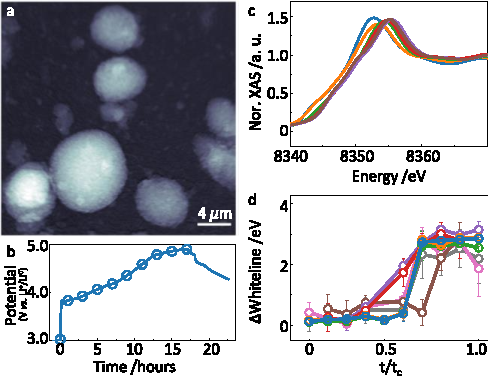
\includegraphics{figures/nca_txm.pdf}
  \caption{Operando \gls{txm} of \nca{} during first charge. (a) Mean
    optical depth frame of \nca{} particles. (b) Applied potential to
    operando cell during galvanostatic charging at
    \SI{0.05}{\ampere\per\ampere\per\hour} (C/20). (c) Normalized spectra
    from \emph{ex-situ} ensemble-average \gls{xas}. (d)
    State-of-charge determined by whiteline position relative to
    overall state of charge in (c) for individual particles of
    \nca{}. Error bars represent one standard deviation over pixels
    within the given particle.}
  \label{fig:txm-nca}
\end{figure}

\begin{figure}[!h]
  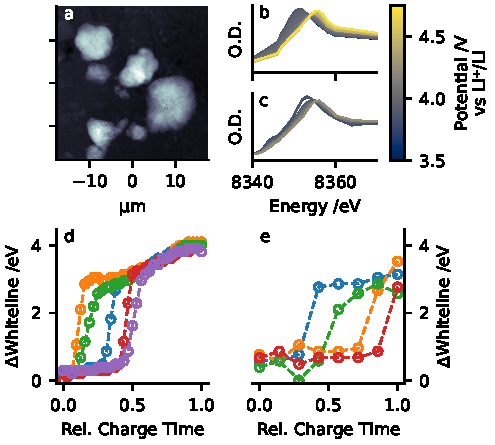
\includegraphics{figures/nmc_txm.pdf}
  \caption{Operando \gls{txm} \gls{xas} of \nmc[333]{} and \nmc[532]{}
    during first charge. (a) Mean optical depth frame of \nmc[333]{}
    particles. (b,c) Median optical depth spectra of active material
    during (b) second charge of \nmc[333]{} and (c) first charge of
    \nmc[532]{}. (d,e) Changes in median whiteline energies during
    first charge relative to start of charging for individual
    particles of (d) \nmc[333]{} (e) \nmc[532]{}.}
  \label{fig:txm-nmc}
\end{figure}

\newpage
\begin{figure}[!h]
    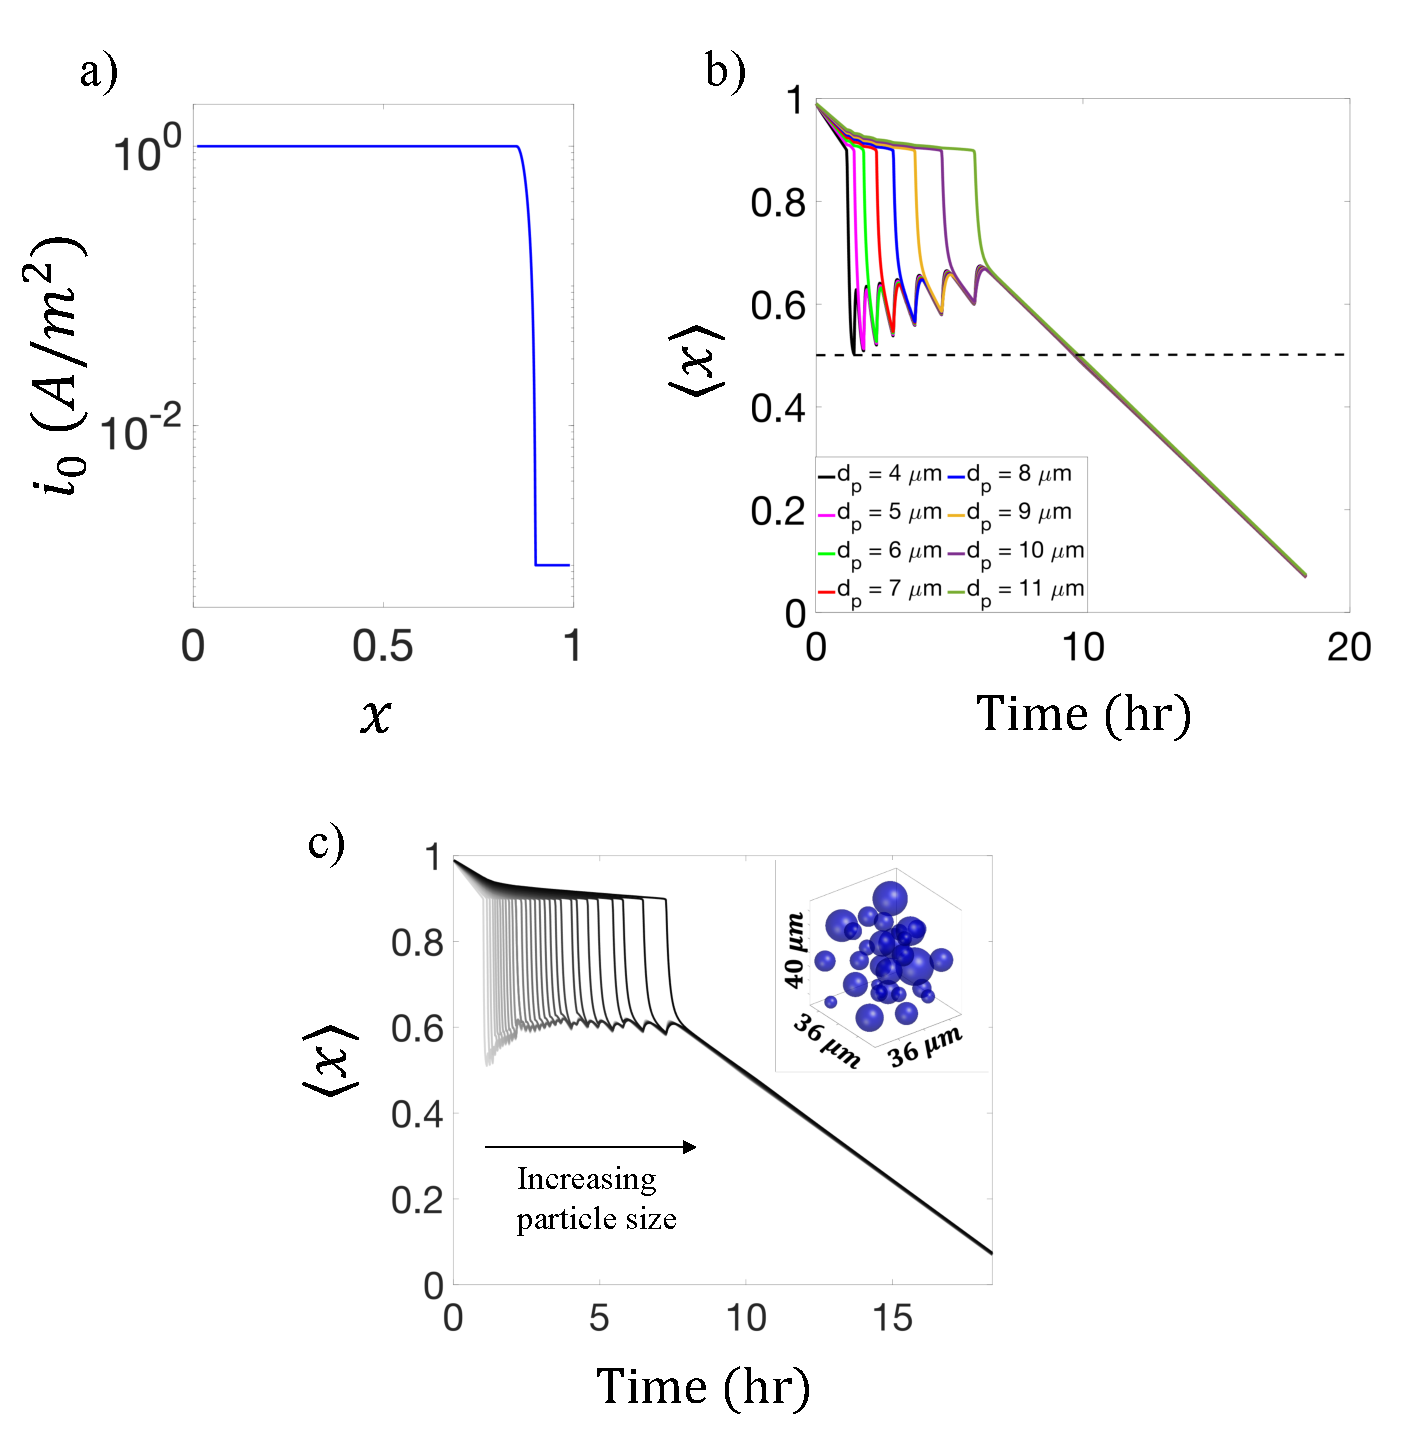
\includegraphics[scale =0.7]{figures/modeling_figure_1.pdf}
    \caption{Simulation results for C/20 galvanostatic charging. (a) The model form of \gls{ecd} vs. $x$ used for the simulation. The evolution of the volume-averaged Li concentration in individual particle, $\langle x \rangle$, for (b) the 8-particle system and (c) 30-particle system.}
    \label{fig:model-1}
\end{figure}

\newpage
\begin{figure}[!h]
    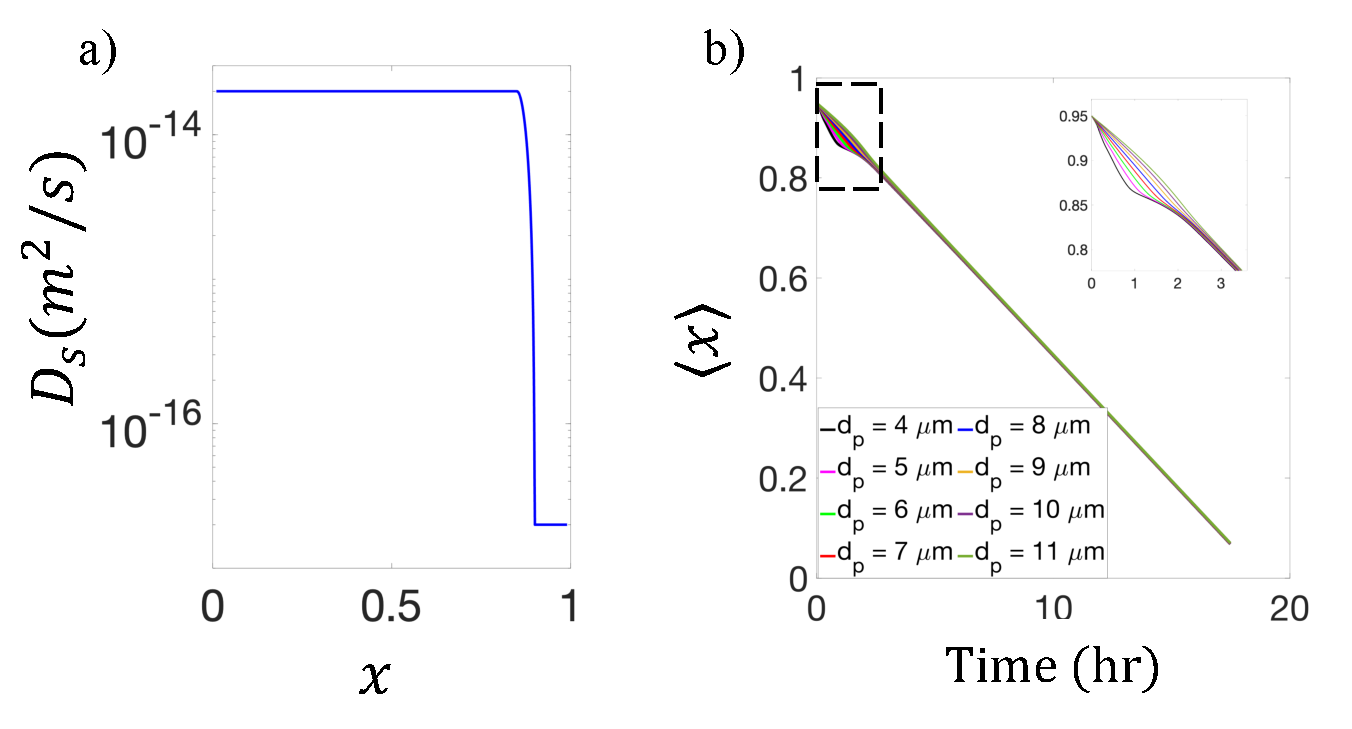
\includegraphics[scale =0.7]{figures/modeling_figure_2_with_Ds_1000_cs_0.95.pdf}
    \caption{Simulation results for C/20 galvanostatic charging. (a) The model form of $D_s$ vs. $x$ used for the simulation. Note that the form is the same in terms of the ratio between minimum and maximum values and the transition-zone width as that of \gls{ecd} shown above. (b) The evolution of the volume-averaged Li concentration in individual particle, $\langle x \rangle$, for the 8-particle system. The inset shows the zoomed in version of the section highlighted using the dashed box.}
    \label{fig:model-2}
\end{figure}


\newpage
\bibliographystyle{plain}
\bibliography{refs,refs-extra}
%% \bibliography{references}

\end{document}
